\documentclass{article}
\usepackage{iclr2027_conference,times}
\usepackage[utf8]{inputenc}
\usepackage[T1]{fontenc}
\usepackage{amsmath,amssymb,amsthm}
\usepackage{booktabs}
\usepackage{graphicx}
\usepackage{hyperref}
\usepackage{url}

\newtheorem{theorem}{Theorem}
\newtheorem{proposition}{Proposition}
\theoremstyle{definition}
\newtheorem{definition}{Definition}
\theoremstyle{remark}
\newtheorem*{remark}{Remark}

\newcommand{\Ev}{\mathcal{E}}
\newcommand{\K}{\mathcal{K}}
\newcommand{\Y}{\mathcal{Y}}
\newcommand{\Ex}{\mathbb{E}}
\newcommand{\R}{\mathbb{R}}
\newcommand{\tr}{\operatorname{tr}}
\newcommand{\dG}{d_{G}}

\title{The Indifference Threshold of a Language-Model Judge\\Is Its Symbol Budget}

\author{Anonymous authors\\Paper under double-blind review}

% \iclrfinalcopy

\begin{document}
\maketitle

\begin{abstract}
An evaluator with finite resolution does not order every pair of options.
Two options whose consequences differ by less than the evaluator can resolve are indifferent, and the induced preference is a semiorder rather than a weak order.
Geometric Evaluation Theory derives that structure from an evaluation object made of a consequence map, a metric with an ideal point, and a resolution budget, and proves that the threshold of the semiorder equals the budget rather than being a free parameter.
We test that prediction on an evaluator the theory did not build.
A language-model judge, Qwen2.5-7B-Instruct, is asked to report how far a number lies from a target, and its preference between two options is the order of its reports.
Three budgets are set independently and registered before the run.
Coarsening the numbers the judge is shown from three decimals to none raises its threshold from 0.0009 to 0.87, at 0.86 to 0.87 of the rendering step at every level.
Limiting the judge's report to two through six generated tokens sets the threshold at 0.87 of the resolution those symbols can express, from 0.87 down to 0.0009.
Quantizing the judge's weights from bfloat16 to 8 bits and to 4 bits leaves every threshold unchanged within the registered tolerance.
Pairs separated by more than twice the largest measured threshold are ordered alike in every cell, with worst-case accuracy 0.985.
The resolution of the judge is the budget of symbols it is shown and allowed to emit, and not the precision of its weights.
The registration, its hash, and the graded record are public.
\end{abstract}

\section{Introduction}

A language model used as a judge is asked to tell two things apart.
It is shown two answers, or two numbers, or two candidates, and asked which is better or how far each is from what was wanted.
The practice is now standard \citep{zheng2023}, and its known failures are position bias, a preference for round scores, and a dependence on the grading scale \citep{li2026grading}.
What has not been asked is the question that precedes all of those.
How fine a difference can the judge resolve at all, and what sets that limit?

This paper answers the question for one judge on one task, under a theory that says what the answer has to be.
The theory is Geometric Evaluation Theory.
It begins one step before a preference ordering.
An evaluator maps actions into a space of consequences, measures them with a metric of its own from an ideal point of its own, and does so at a finite resolution.
The distinctions it can make are derived first, and preference and choice follow from them.
At infinite resolution the induced preference is a weak order with a utility.
At finite resolution it is a semiorder in the sense of \citet{luce1956}, an ordering with intransitive indifference, and the theory proves that the threshold of that semiorder is the resolution budget itself.
Luce took the threshold as a primitive.
Here it is a measurable property of the evaluator, fixed by the object that defines it, and that makes the claim one a measurement can fail.

We ran that measurement under a registration sealed before the data were read.
The judge is Qwen2.5-7B-Instruct \citep{qwen2025}, shown a target and a value and asked how far apart they are.
Its consequence map is known exactly, since the consequence of a value is its distance from the target.
Three budgets were set independently.
The judge was shown the numbers at zero to three decimals, was allowed one to twelve tokens for its report, and was run at bfloat16, 8-bit, and 4-bit weights.
The prediction is that the threshold tracks each output budget where the budget exceeds the judge's own floor, and that pairs far apart keep their order in every cell.

Three things were found.
The threshold tracked the rendering step at 0.86 to 0.87 of the step over three orders of magnitude, and tracked the resolution afforded by the report length at 0.87 over the same range.
Reducing the weights to 8 and then to 4 bits moved no threshold beyond the registered tolerance.
Pairs separated by 20 were ordered the same way in every one of eighteen cells at an accuracy of at least 0.985.
The judge's resolution is the budget of symbols it is shown and allowed to emit.
Its weight precision is, on this task, not a resolution budget at all.

The paper also reports two supporting gates run under sealed registrations and one that returned indeterminate.
A hull law that every evaluator of this kind must obey was tested on a public survey with a known consequence map and held as a population tendency and not as a deterministic law.
The theory's identification theorem was tested on synthetic evaluators and passed in every cell.
A regret bound for evaluators that share one representation was tested on the grouped-query attention of a language model and could not be graded, for a reason we state.
The registrations, their hashes, and the graded records are provided as supplementary material.

\section{The evaluation object}
\label{sec:object}

\begin{definition}[Evaluation object]
\label{def:object}
An evaluation object is a six-tuple $\Ev=(X,A,C,G,B,\K)$ in which $X$ is a set of states carrying a probability law $\mu$, the evaluator's belief; $A$ is a set of actions; $C:A\times X\to\Y$ is the evaluator, a map into a consequence space $\Y$ that is a $C^{1}$ manifold; $G$ is the metric of evaluation, a continuous Riemannian metric on $\Y$ together with an ideal point $t\in\Y$; $B$ is the resolution budget, one of a rank cap $k$, a length $\varepsilon\ge0$, or a rate $R$ in bits, with $B=\infty$ for the unbudgeted case; and $\K\subseteq A$ is the set of admissible actions.
\end{definition}

The world supplies $(X,A,C)$ and the evaluator supplies $(G,B,\K)$.
Two evaluators of the same world differ only in the second triple.
The split is the source of the theory's content.
If the evaluator could also choose $C$, every weak order on a finite $A$ would be an evaluation object, since a one-dimensional consequence $C(a)=t-d(a)$ represents any real function $d$.
With $C$ fixed by the world, which preferences an evaluator can hold becomes a representation theorem and what its choices reveal becomes a uniqueness theorem.

The evaluation distance of an action is the expected geodesic distance of its consequence from the ideal, $d(a)=(\Ex_{\mu}[\dG(C(a,X),t)^{2}])^{1/2}$, and its cost is $c(a)=d(a)^{2}$.
Under a rank cap $k$ the evaluator retains the top-$k$ eigenspace of the second moment of its habitual consequences and evaluates the projection.
Under a length $\varepsilon$ the distance is $d$ itself and the budget acts on comparison.
Under a rate $R$ the evaluator holds an $R$-bit description of the consequence and evaluates the reconstruction, and a rate budget is treated as the length budget given by the least attainable distortion.
The length budget is the one this paper measures.

\section{What the object induces}
\label{sec:derive}

\begin{theorem}[Induced distinctions]
\label{thm:dist}
Let $\Ev$ be an evaluation object.
(a) The relation $a\sim b$ if and only if $C(a,x)=C(b,x)$ for $\mu$-almost every $x$ is an equivalence relation on $A$.
(b) Under a rank cap $k$ the relation $a\sim_{k}b$ if and only if the retained projections of $C(a,\cdot)$ and $C(b,\cdot)$ agree almost everywhere is an equivalence relation each of whose classes is a union of classes of $\sim$.
(c) Under a length $\varepsilon$ the relation $a\approx_{\varepsilon}b$ if and only if $|d(a)-d(b)|\le\varepsilon$ is reflexive and symmetric, and it is transitive on $A$ if and only if $\varepsilon=0$ or the set $\{d(a)\}$ contains no three points $r_{1}<r_{2}<r_{3}$ with $r_{2}-r_{1}\le\varepsilon$, $r_{3}-r_{2}\le\varepsilon$, and $r_{3}-r_{1}>\varepsilon$.
\end{theorem}

Part (c) is the whole difference between a resolution budget and a rank budget.
A rank budget coarsens the evaluator's world into classes.
A length budget produces a tolerance, and the failure of transitivity is the signature of finite resolution rather than a defect of the evaluator.

\begin{definition}[Induced preference]
\label{def:pref}
Write $d_{B}$ for the budgeted distance and $\varepsilon_{B}$ for the length budget, with $\varepsilon_{B}=0$ under a rank cap or no budget.
Then $a\succ_{B}b$ if and only if $d_{B}(a)+\varepsilon_{B}<d_{B}(b)$, and $a\sim_{B}b$ if and only if $|d_{B}(a)-d_{B}(b)|\le\varepsilon_{B}$.
\end{definition}

\begin{theorem}[Preference from geometry]
\label{thm:pref}
Let $A$ be finite.
(a) For $\varepsilon_{B}=0$ the relation $\succsim_{B}$ is a weak order represented by the utility $u_{B}=-d_{B}$, unique up to strictly increasing transformation.
(b) For $\varepsilon_{B}>0$ the pair $(\succ_{B},\sim_{B})$ is a semiorder in the sense of Luce, and $u_{B}=-d_{B}$ with threshold $\varepsilon_{B}$ is a threshold representation of it.
(c) The semiorder of (b) is a weak order if and only if the condition of Theorem~\ref{thm:dist}(c) holds, and as $\varepsilon_{B}\to0$ it converges to the weak order of (a).
\end{theorem}

Proofs are in Appendix~\ref{app:proofs}.
\citet{luce1956} derived semiorders from just-noticeable differences in utility with the threshold as a primitive, \citet{scott1958} gave the representation, and \citet{fishburn1970} and \citet{tversky1969} the extensions and the evidence.
Here the threshold is the budget and the utility is the distance to the ideal, so both are fixed by the evaluation object.
A semiorder with intransitive indifference is what a finite-resolution evaluator must exhibit, and its threshold is a measurable property of the evaluator rather than a fitted constant.
That sentence is the prediction Section~\ref{sec:test} tests.

Choice from a menu is the set of admissible actions no admissible action strictly beats, which is nonempty on a finite menu because a semiorder is acyclic.
Under a length budget every admissible action within $\varepsilon$ of the least distance is chosen, which is satisficing \citep{simon1955} with the aspiration level as the ideal and the tolerance as the budget.

\begin{theorem}[Representation, hull law, uniqueness]
\label{thm:repr}
Let $X$ be a point, $\Y=\R^{m}$, and the consequences $y_{a}=C(a)$ fixed by the world, with the evaluator choosing a positive semidefinite $G$ and an ideal $t$, so that $c(a)=(y_{a}-t)^{\top}G(y_{a}-t)$.
(a) A weak order on finite $A$ is representable by some $(G,t)$ if and only if a semidefinite feasibility problem with $|A|(|A|-1)/2$ linear constraints has a solution.
(b) If a preference is representable, then for every action $a$ and finite set $S$ with $y_{a}$ in the convex hull of $\{y_{s}:s\in S\}$ there is $s\in S$ with $a\succsim s$. No action is strictly worse than every action whose consequences surround it, and this holds for every convex evaluation cost.
(c) If two evaluations $(G_{1},t_{1})$ and $(G_{2},t_{2})$ with $G_{1}\neq0$ induce the same weak order on a nonempty open connected set of consequences, then $G_{2}=\lambda G_{1}$ for some $\lambda>0$ and $G_{1}(t_{2}-t_{1})=0$.
\end{theorem}

Part (b) is the first law of the theory that a scalar utility does not state, and it is checkable on data whenever the consequence map is known.
Part (c) says what choices can identify, the metric up to scale and the ideal up to the metric's kernel, and no more.
A rank budget also produces a reversal that no single utility records: there is an object and two actions with $b\succ a$ at rank cap 1 and $a\succ b$ at rank cap 2, with the same metric and the same ideal at both budgets (Appendix~\ref{app:proofs}).

\section{The test: a judge with a known consequence map}
\label{sec:test}

The prediction is that for a fixed world and evaluator the indifference threshold of the induced semiorder is the resolution budget.
Coarsening the resolution at which the evaluator resolves consequences enlarges the threshold, and the ordering of pairs separated by more than the largest threshold does not change.
The test needs an evaluator whose consequence map is known and whose budget can be set from outside.
A language-model judge on a numeric task is such an evaluator, and it is one the theory did not build.

\paragraph{Evaluator.}
Qwen2.5-7B-Instruct \citep{qwen2025}, at a recorded revision, loaded in bfloat16, in 8-bit \citep{dettmers2022}, and in 4-bit NF4 \citep{dettmers2023}.
The judge is a scorer.
Shown, in its chat template, a target value and one value, it is asked how far the value is from the target and answers with a number, read as the first number in its greedy generation.
The prompt is ``Target: $\{$target$\}$. Value: $\{$value$\}$. How far is the value from the target? Answer with a single number and nothing else.''
The induced preference between two options compares their reported distances.
Equal reports, and any unparsable report, are indifference.
This is the theory's evaluator, a map from a consequence to a scalar cost whose order is the preference, and the model's own output resolution and arithmetic are its floor.

Two earlier instruments were tried on a probe seed and are kept in the record.
A pairwise chooser asked which of two options is closer, read from the next-token logits of the answer letters with both orders shown.
With options on either side of the target it was vacuous, choosing the larger number in every straddling pair.
With options on one side it reached accuracy 0.99 at a gap of 10 but stayed between 0.43 and 0.63 from gap 0.01 to gap 2, because its first-position preference held the two-order average near one half until the gap was large.
A pairwise chooser measures its position bias before it measures a threshold, so it was replaced by the scorer before any pilot.

\paragraph{Consequences.}
The target is 100.
An option is a number in $[50,150]$ and its consequence is its distance from the target, between 10 and 40, two digits before the decimal point so that a report of fixed length has fixed resolution.
A pair is two options whose distances differ by a gap on the ladder 0.0005, 0.001, 0.002, 0.005, 0.01, 0.02, 0.05, 0.1, 0.2, 0.5, 1, 2, 5, 10, 20, each option on either side of the target with equal probability, 200 pairs per gap drawn by seed.

\paragraph{Budgets.}
Three, set independently.
Rendering precision: the numbers are shown with 0, 1, 2, or 3 decimals, the target at the same precision, so that at $d$ decimals two options whose distances differ by less than $10^{-d}$ may render identically.
Report length: the scorer's answer is limited to $k$ generated tokens, $k$ in 1, 2, 3, 4, 5, 6, 12.
This tokenizer emits one digit per token, so with two-digit distances a report of $k$ tokens resolves 10 at $k=1$, 1 at $k=2$ and $k=3$ (the third character is the decimal point), 0.1 at $k=4$, 0.01 at $k=5$, and 0.001 from $k=6$.
This is the theory's length budget taken literally.
The evaluator may spend $k$ symbols on its cost, and the threshold should be the resolution those symbols afford.
Weight precision: bfloat16, 8-bit, 4-bit.
The cells are rendering by weight precision at full report length, twelve cells, and the report ladder at three decimals and full weights, six more.

\paragraph{Estimator.}
For each cell and gap, accuracy is the share of pairs whose preference for the closer option exceeds one half, with ties and unparsable reports counting as one half so that indifference counts against.
The threshold of a cell is the gap at which accuracy first reaches 0.9, interpolated linearly in log gap between ladder points, infinite if never reached and the smallest gap if reached there.
A self-test on a scorer that rounds to a grid of step $h$ recovered thresholds 0.0088, 0.087, and 0.87 at $h=0.01$, $0.1$, and $1$.
That is where the 90 percent level of a rounding scorer sits, since a pair a fraction of a step apart rounds to the same value with a probability that falls linearly in the gap.

\paragraph{Predictions and bars.}
The scorer's threshold in a cell is the larger of the budget it was set and a floor, the scorer's own resolution at full weights, full rendering, and full report length.
P1: along the rendering ladder at fixed weight precision the threshold is non-increasing in decimals within a tolerance factor, and at every decimal count whose step exceeds the floor by a factor of at least 3 it is within that factor of the step.
P1b: the same along the report ladder for $k\ge2$, with the $k=1$ cell reported and not graded because its resolution of 10 sits at the edge of the gap ladder.
P2: along the weight ladder at three decimals and full report length the threshold is non-decreasing as bits are removed, within the factor.
P3: for every gap at least twice the largest threshold measured in any cell, accuracy is at least 0.95 in every cell.
An anti-vacuity rule required accuracy of at least 0.95 at gap 20 and a floor of at most 0.3 at full precision, so that at least two rendering steps and three report budgets exceed three times the floor.
The tolerance factor was fixed at 1.5 from a pilot on a separate seed.
The registration records that at full weights the rendering and report ladders test only that the scorer's arithmetic resolves what it is shown and allowed to say, which a competent model makes nearly a tautology, and that the weight ladder is where the prediction can fail.

\paragraph{Discipline.}
The registration, with its hypothesis, world, statistic, bars, exclusions and null, was committed and its hash recorded before the run seed was drawn.
The self-test, the probes, and the pilot were run and recorded before sealing, and the run was graded by a script against the sealed bars.
A registration that could pass on empty cells is not sealed, and every probe is cited in it.

\section{Results}
\label{sec:results}

\begin{figure}[t]
\centering
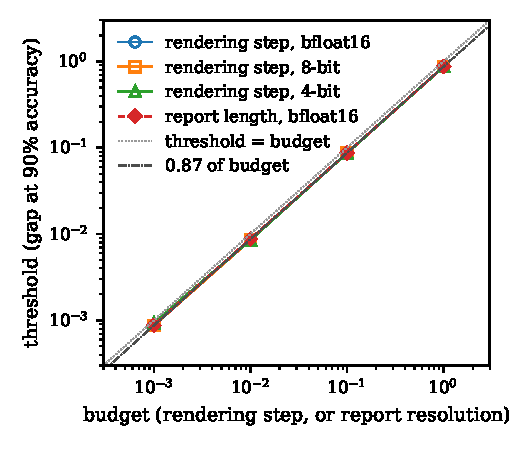
\includegraphics[width=0.58\columnwidth]{figures/thresholds.pdf}
\caption{The threshold tracks the output budget.
Each point is the gap at which the judge reaches 90 percent accuracy in one cell, against the budget set in that cell: the rendering step at three weight precisions, and the resolution afforded by the report length.
Every point lies on the line at 0.87 of the budget, which is where a scorer that rounds to the budget's grid reaches 90 percent.
The three weight precisions coincide.}
\label{fig:thresholds}
\end{figure}

\begin{figure}[t]
\centering
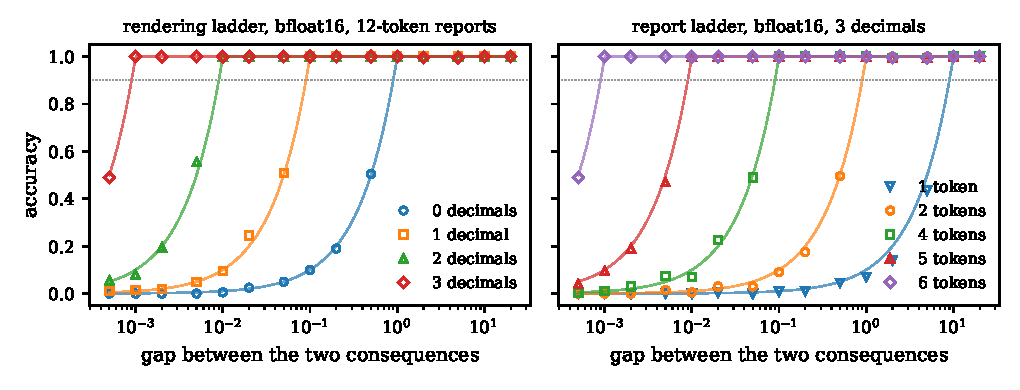
\includegraphics[width=\columnwidth]{figures/accuracy.pdf}
\caption{Accuracy against gap, bfloat16 weights.
Left, the rendering ladder at full report length.
Right, the report ladder at three decimals.
Each curve rises from indifference to ceiling within one decade, and the decade shifts by one order of magnitude with each step of the budget.
The dotted line is the 90 percent level that defines the threshold.}
\label{fig:accuracy}
\end{figure}

\begin{table}[t]
\centering
\small
\caption{Thresholds by cell, the gap at 90 percent accuracy.
Rendering cells at 12-token reports; report cells at 3 decimals and bfloat16.
The budget column is the rendering step or the resolution the report length affords.
Every graded threshold sits between 0.86 and 0.88 of its budget.}
\label{tab:thresholds}
\begin{tabular}{lrrrr}
\toprule
Rendering (decimals) & budget & bfloat16 & 8-bit & 4-bit \\
\midrule
0 & 1 & 0.869 & 0.869 & 0.869 \\
1 & 0.1 & 0.0868 & 0.0868 & 0.0868 \\
2 & 0.01 & 0.00856 & 0.00856 & 0.00856 \\
3 & 0.001 & 0.00087 & 0.00087 & 0.00093 \\
\midrule
Report (tokens) & budget & bfloat16 & & \\
\midrule
1 & 10 & 8.85 (not graded) & & \\
2 & 1 & 0.872 & & \\
3 & 1 & 0.872 & & \\
4 & 0.1 & 0.0873 & & \\
5 & 0.01 & 0.00877 & & \\
6 & 0.001 & 0.00087 & & \\
12 & 0.001 & 0.00087 & & \\
\bottomrule
\end{tabular}
\end{table}

The sealed verdict is a pass on P1, P1b, P2 and P3.
Table~\ref{tab:thresholds} gives every threshold and Figures~\ref{fig:thresholds} and \ref{fig:accuracy} show them against the budgets and the accuracy curves they were read from.
No report was unparsable in any cell.

\paragraph{The threshold tracks the rendering step.}
At bfloat16 the threshold was 0.869, 0.0868, 0.00856, and 0.00087 at 0, 1, 2, and 3 decimals, against rendering steps of 1, 0.1, 0.01, and 0.001.
The ratio to the step is 0.869, 0.868, 0.856, and 0.873.
The floor at full precision is 0.00087, which is the three-decimal step's ratio, so at three decimals the budget and the floor coincide and the cell is where the floor was measured.
The accuracy curves in Figure~\ref{fig:accuracy} show the mechanism.
At $d$ decimals two distances closer than $10^{-d}$ render identically a share of the time recorded per gap, the judge then reports the same number for both, and indifference counts against.
Accuracy rises from near zero to ceiling within a single decade of gap, and the decade is the rendering step.

\paragraph{The threshold tracks the report length.}
At 2, 3, 4, 5, and 6 tokens the threshold was 0.872, 0.872, 0.0873, 0.00877, and 0.00087, against afforded resolutions of 1, 1, 0.1, 0.01, and 0.001.
The ratio is 0.872 to 0.877 at every graded length.
Two and three tokens give the same threshold because the third character is the decimal point, and six and twelve tokens give the same threshold because the floor is reached.
The one-token cell, reported and not graded, gave 8.85 against an afforded resolution of 10.
This is the length budget of Definition~\ref{def:object} taken literally.
The judge may spend $k$ symbols on its cost, and its just-noticeable difference is the resolution of those symbols, at the same 0.87 that the rendering step produces.

\paragraph{Weight precision does not move the threshold.}
At 8-bit weights every rendering-ladder threshold equals its bfloat16 value to the digits shown.
At 4-bit weights the thresholds at 0, 1, and 2 decimals equal the bfloat16 values and the three-decimal threshold is 0.00093 against 0.00087, a ratio of 1.06 inside the registered tolerance of 1.5.
The 4-bit judge at three decimals is a different evaluator in one visible way.
Its accuracy at gaps above the threshold sits at 0.95 to 0.98 rather than at 0.99 to 1.00, a lapse that the 8-bit and bfloat16 judges do not show.
That lapse did not move the threshold, and P3 held in the cell.
The registration named the weight ladder as the place where the prediction could fail, and it did not.

\paragraph{Well-separated pairs keep their order.}
The largest threshold in any cell is 8.85, in the one-token cell, so the only ladder gap at least twice that is 20.
At gap 20 the worst accuracy over all eighteen cells is 0.985.
A budget change enlarged the indifference threshold by four orders of magnitude and reordered nothing that was resolved at every budget.

\section{Supporting gates}
\label{sec:gates}

Three further predictions of the theory were run under sealed registrations of the same discipline.
Each is reported at the size of its verdict.

\paragraph{Hull law on a public survey, pass as a tendency.}
Theorem~\ref{thm:repr}(b) needs only a known consequence map and observed choices.
In the 1972 American National Election Study respondents placed candidates and parties on seven-point issue scales and rated them on feeling thermometers, so the consequence of an object is its position on a registered pair of scales and the choice is the rating.
On the registered pair, 489 of 557 respondents had a menu in which the law could bind, and 246 of them, 50.3 percent, violated it at least once, against 66.4 percent when each respondent's ratings are shuffled among that respondent's own objects, with none of 200 shuffles reaching the observed rate.
Five other pairs of scales gave the same ordering, observed rates of 54 to 63 percent against shuffled rates of 67 to 74 percent.
The rates sit well below the geometric base rate of violation and well above zero.
On this world the law holds as a population tendency and fails as the deterministic statement of the theorem for about half of the respondents, and the registration records both halves.

\paragraph{Identification on synthetic evaluators, pass.}
Theorem~\ref{thm:repr}(c) says what choices can recover.
Forty evaluators per cell, in two to four dimensions with random metrics including singular ones, were given batteries of consequences of increasing size, and the feasibility program of Theorem~\ref{thm:repr}(a) with a margin was solved from their weak orders alone.
Errors were scored against the chance level of guesses from the evaluator prior.
In all twelve cells on a fresh seed the metric and the ideal's range component were recovered at 64 consequences above the dimension, to a few percent of chance, with the error falling at every step as the battery grew, while at or below the design bound, off the span of a battery confined to a subspace, and in the kernel of a singular metric, nothing was recovered.
A semiorder that withholds the fifth of pairs closest in distance identified more slowly, to between 5 and 25 percent of chance at the same battery.

\paragraph{Shared-representation regret, indeterminate.}
When several evaluators must read one representation of fixed rank, the theory computes each one's regret and says the least total regret is attained by the leading eigenspace of the influence-weighted sum of their geometries (Appendix~\ref{app:incompat}).
The gate took the three query heads of a grouped-query attention group in a language model as evaluators of one key cache, with shared codes of rank 2, 4, and 8 in 128 dimensions.
At those ranks the measured attention loss was 20 to 330 times the second-order prediction, so the regret formula and its bound could not be tested and the verdict is indeterminate.
The ordering claim survived on the measured losses alone.
The leading eigenspace of the summed geometries beat every random code and the key-covariance code in 32 of 32 cases, while a head's own leading eigenspace was the best code for that head in fewer than half the cases.
A second sealed run perturbed one key at a time by a small isotropic error in the discarded subspace and there the measured loss matched the second-order prediction at the median, a ratio of 1.02 to 1.05, while 64 draws per cell left a 20 percent scatter that missed the registered per-triple bar, so that verdict is indeterminate as well.
The registration of the first run also compared a one-key prediction to an all-keys measurement, a defect we record rather than repair after the fact.

\section{Related work}
\label{sec:related}

Finite resolution producing intransitive indifference is Luce's semiorder \citep{luce1956}, with the representation of \citet{scott1958} and the evidence of \citet{tversky1969}.
The present theory adds that the threshold is the budget and the utility is a distance from an ideal, both fixed by the evaluation object, so the semiorder's parameter is measurable rather than fitted.
The core of the induced preference, a weighted distance from an ideal point, is Coombs' unfolding \citep{coombs1964} and the spatial theory of voting \citep{davis1970,enelow1984}, whose weight matrix is a constant metric of evaluation.
Those models are the unbudgeted, single-evaluator case of the object.
The nearest neighbor with a budget is rational inattention and limited attention \citep{sims2003,caplin2015,masatlioglu2012,matejka2015}, in which a cost of information about the state produces consideration sets and stochastic choice.
The budget here is a different quantity.
It limits the resolution of consequences under the evaluator's metric, not the acquisition of information about states, and its predictions are not statements those models make.
The decision geometry of \citet{dawid2007} derives a geometry on distributions from a scoring rule and is the case of an identity evaluator with the true distribution as ideal and no budget.
The pullback construction that gives an evaluator its geometry, and the regret bound of Appendix~\ref{app:incompat}, come from a companion draft on observer representation \citep{bond2026or}, and the economics application is in \citet{bond2026tcss}.

On language-model judges, \citet{zheng2023} established the practice and its position and verbosity biases, and \citet{li2026grading} found human alignment highest on a 0 to 5 scale, with finer scales worse.
That finding is about the scale a judge is asked to use.
The present result is about the resolution the judge has, and it says that the resolution is set by the symbols on both sides of the judge, what it is shown and what it may emit, at a constant fraction of their grid.
On quantization, \citet{lee2025quant} report that 4-bit weights cost small models accuracy on hard tasks and on MT-Bench conversation quality.
Our 4-bit judge showed a lapse of a few percent above its threshold and no change in the threshold, on a task where the consequence map is known and the resolution is set from outside.
The two findings measure different quantities and we do not read ours against theirs.

\section{Scope}
\label{sec:scope}

The result is one model on one numeric task with a known consequence map.
At full weights the rendering and report ladders test whether the judge's arithmetic resolves what it is shown and allowed to say, and a competent model makes that nearly a tautology.
The informative parts are the weight ladder, where the prediction could have failed and did not, and the ordering of well-separated pairs across a four-order-of-magnitude change in threshold.
The 0.87 is a property of a rounding scorer's accuracy curve at the 90 percent level, and a different level would give a different constant at the same budget.
Nothing here is a claim about human evaluators.
A human budget manipulation is registered as a later gate and waits on ethics review.
The hull law held on the survey as a tendency and not as a law, and the regret bound could not be tested at the ranks tried.
What would fail the threshold claim is stated in the registration: a threshold that does not move with resolution where the theory says it must, one that shrinks when resolution is coarsened, or a reordering of well-separated pairs.

\subsection*{AI use statement}
Generative AI tools were used for drafting and editing text, for writing experiment and analysis code, and for literature search.
They were not used to generate research ideas, data, or results, and no reported number was produced by a generative model.
All AI-assisted work was reviewed by the authors.
Code was tested against a self-test with known answers before any registered run, and every citation was checked against the publisher's record.
The authors take responsibility for the final content of this work, including text, claims, and artifacts produced with the aid of generative AI.

\subsection*{Ethics statement}
The survey data are a public-use release of the American National Election Studies with no identifiers.
No human subjects were run.
The registered human gate will be submitted for institutional review before any participant is recruited.

\subsection*{Reproducibility statement}
The supplementary material contains, for every gate, the sealed registration with its hash, the configuration with model revision and library versions, the seeds, the run log, the graded record, and the grading script that applies the sealed bars.
Proofs of every theorem are in Appendix~\ref{app:proofs}.
The judge is an openly released model at a recorded revision, and the stimulus generator, the scorer prompt, and the estimator are given in full in Section~\ref{sec:test} and in the supplementary code.

\bibliography{refs}
\bibliographystyle{iclr2027_conference}

\appendix

\section{Proofs}
\label{app:proofs}

\begin{proof}[Proof of Theorem~\ref{thm:dist}]
(a) Equality almost everywhere is an equivalence relation.
(b) The relation is equality of a function of $a$, hence an equivalence, and $C(a,x)=C(b,x)$ implies equality of the retained projections, so each $\sim_{k}$ class contains the $\sim$ classes of its members.
(c) Reflexivity and symmetry are immediate.
If three such points exist then $r_{1}\approx_{\varepsilon}r_{2}$ and $r_{2}\approx_{\varepsilon}r_{3}$ but not $r_{1}\approx_{\varepsilon}r_{3}$.
If none exist, take $a\approx_{\varepsilon}b\approx_{\varepsilon}c$ with values $r_{a},r_{b},r_{c}$.
If $r_{a}\le r_{b}\le r_{c}$ or the reverse, the absence of such a triple gives $|r_{a}-r_{c}|\le\varepsilon$, and in every other ordering $|r_{a}-r_{c}|\le\max(|r_{a}-r_{b}|,|r_{b}-r_{c}|)\le\varepsilon$.
\end{proof}

\begin{proof}[Proof of Theorem~\ref{thm:pref}]
(a) A relation defined by comparing a real function is complete and transitive, and the function represents it. Uniqueness up to monotone transformation is the standard ordinal uniqueness.
(b) A relation defined by $u(a)>u(b)+\varepsilon$ with fixed $\varepsilon>0$ is irreflexive and satisfies the two semiorder axioms.
If $a\succ b$ and $c\succ e$, then $u(a)>u(b)+\varepsilon$ and $u(c)>u(e)+\varepsilon$, so either $u(a)>u(e)+\varepsilon$ or $u(c)>u(b)+\varepsilon$, since if both failed we would have $u(a)\le u(e)+\varepsilon<u(c)$ and $u(c)\le u(b)+\varepsilon<u(a)$, a contradiction.
If $a\succ b\succ c$ and $e$ is any action, then $u(a)>u(c)+2\varepsilon$, so either $u(a)>u(e)+\varepsilon$ or $u(e)\ge u(a)-\varepsilon>u(c)+\varepsilon$.
This is the easy direction of the Scott and Suppes representation of semiorders, and the representation is by construction.
(c) The semiorder is a weak order exactly when indifference is transitive, which is Theorem~\ref{thm:dist}(c), and for finite $A$ the condition holds for all sufficiently small $\varepsilon$.
\end{proof}

\begin{proof}[Proof of Theorem~\ref{thm:repr}]
(a) Expanding, $q(y)=(y-t)^{\top}G(y-t)=y^{\top}Gy-2t^{\top}Gy+t^{\top}Gt$, which is a quadratic $Q(y)=y^{\top}Gy+b^{\top}y+\gamma$ with $b=-2Gt$ in the range of $G$.
Conversely, given such $Q$ with $b$ in the range of $G$, choose $t$ with $Gt=-b/2$, and then $Q$ differs from $q$ by a constant, so the two order $A$ identically.
The constraints $Q(y_{a})<Q(y_{b})$ for $a\succ b$ and $Q(y_{a})=Q(y_{b})$ for $a\sim b$ are linear in the entries of $(G,b,\gamma)$ for fixed consequences, the positive semidefinite cone is convex, and the range condition is the linear constraint that $b$ be orthogonal to the kernel of $G$, so the problem is a semidefinite feasibility problem.
(b) $q$ is convex because $G$ is positive semidefinite.
If $y_{a}=\sum_{s}\lambda_{s}y_{s}$ with $\lambda_{s}\ge0$ summing to one, then $q(y_{a})\le\sum_{s}\lambda_{s}q(y_{s})\le\max_{s}q(y_{s})$, so $a\succsim s^{*}$ for a maximizer $s^{*}$.
The argument used only convexity.
(c) Same weak order on $U$ means $q_{2}=\varphi\circ q_{1}$ on $U$ for a strictly increasing $\varphi$ on $q_{1}(U)$, an interval because $U$ is connected and $q_{1}$ continuous.
Along any line segment in $U$ on which $q_{1}$ is not constant, $q_{1}(s)=\alpha(s-s_{0})^{2}+\beta$ with $\alpha>0$, symmetric about $s_{0}$, and $q_{2}(s)=\varphi(q_{1}(s))$ is a quadratic in $s$ also symmetric about $s_{0}$, so $\varphi$ is affine with positive slope on the interval $q_{1}$ traces along the segment.
Two such segments through a common point trace overlapping intervals, an affine function is determined by its values on an interval, and $U$ is connected, so $\varphi(u)=\lambda u+\mu$ with $\lambda>0$ on all of $q_{1}(U)$.
Then $q_{2}=\lambda q_{1}+\mu$ on an open set, two polynomials that agree on an open set agree identically, and comparing quadratic and linear parts gives $G_{2}=\lambda G_{1}$ and $G_{1}(t_{2}-t_{1})=0$.
\end{proof}

\begin{proof}[Resolution reversal]
Take $\Y=\R^{2}$, $G=I$, $t=0$, $X$ a point, and a workload whose consequence second moment has top eigenvector $e_{1}$, for example $\operatorname{diag}(4,1)$.
Let $C(a)=(1,0)$ and $C(b)=(0.9,2)$.
Then $d_{1}(a)=1$, $d_{1}(b)=0.9$, $d_{2}(a)=1$, and $d_{2}(b)=\sqrt{0.81+4}=2.19$, so $b\succ a$ at rank cap 1 and $a\succ b$ at rank cap 2.
A function representing both would satisfy $u(b)>u(a)$ and $u(a)>u(b)$.
\end{proof}

\section{Coupled evaluators}
\label{app:incompat}

Let $N$ evaluators share a representation space $\R^{d}$ with constant pullbacks $P_{1},\dots,P_{N}$ and a common isotropic source of second moment $\sigma^{2}I$, and let a shared representation at budget $k$ be an orthogonal projector $\Pi$ of rank $k$.
Evaluator $i$'s regret from $\Pi$ is $r_{i}(\Pi)=\sigma^{2}(\sum_{j\le k}\lambda_{j}(P_{i})-\tr(\Pi P_{i}))\ge0$.
A shared representation with zero regret for every evaluator exists if and only if there is a $k$-dimensional subspace that is a top-$k$ eigenspace of every $P_{i}$.
For weights $w_{i}>0$ the least weighted total regret is attained by a top-$k$ eigenspace of $\bar P=\sum_{i}w_{i}P_{i}$ and equals $\sigma^{2}(\sum_{i}w_{i}\sum_{j\le k}\lambda_{j}(P_{i})-\sum_{j\le k}\lambda_{j}(\bar P))$, strictly positive exactly when no common eigenspace exists.
Both statements are Ky Fan's maximum principle \citep{fan1949} applied to $\tr(\Pi P_{i})$ and to $\tr(\Pi\bar P)$.
The regret formula itself is the second-order expansion of the loss under a rank-$k$ code, which is why a measured loss far from quadratic, as in Section~\ref{sec:gates}, leaves the bound untested.

\section{Per-cell accuracy}
\label{app:cells}

Table~\ref{tab:cells} gives the accuracy at every ladder gap in every cell of the run, from which each threshold in Table~\ref{tab:thresholds} was read.

\begin{table}[h]
\centering
\scriptsize
\caption{Accuracy by gap for all eighteen cells. Columns are the gap ladder. Cells are weight precision, decimals, report tokens.}
\label{tab:cells}
\setlength{\tabcolsep}{3pt}
\begin{tabular}{lrrrrrrrrrrrrrrr}
\toprule
cell & .0005 & .001 & .002 & .005 & .01 & .02 & .05 & .1 & .2 & .5 & 1 & 2 & 5 & 10 & 20 \\
\midrule
bf16, 0, 12 & 0.00 & 0.00 & 0.00 & 0.00 & 0.01 & 0.03 & 0.05 & 0.10 & 0.19 & 0.51 & 1.00 & 1.00 & 1.00 & 1.00 & 1.00 \\
bf16, 1, 12 & 0.01 & 0.01 & 0.02 & 0.05 & 0.10 & 0.24 & 0.51 & 1.00 & 1.00 & 1.00 & 1.00 & 1.00 & 1.00 & 1.00 & 1.00 \\
bf16, 2, 12 & 0.06 & 0.08 & 0.20 & 0.56 & 1.00 & 1.00 & 1.00 & 1.00 & 1.00 & 1.00 & 1.00 & 1.00 & 1.00 & 1.00 & 1.00 \\
bf16, 3, 12 & 0.49 & 1.00 & 1.00 & 1.00 & 1.00 & 1.00 & 1.00 & 1.00 & 1.00 & 1.00 & 1.00 & 0.99 & 0.99 & 1.00 & 1.00 \\
bf16, 3, 1 & 0.00 & 0.00 & 0.00 & 0.00 & 0.00 & 0.01 & 0.00 & 0.01 & 0.01 & 0.04 & 0.07 & 0.14 & 0.43 & 1.00 & 1.00 \\
bf16, 3, 2 & 0.00 & 0.00 & 0.00 & 0.01 & 0.01 & 0.03 & 0.03 & 0.09 & 0.17 & 0.49 & 1.00 & 1.00 & 1.00 & 1.00 & 1.00 \\
bf16, 3, 3 & 0.00 & 0.00 & 0.01 & 0.02 & 0.01 & 0.03 & 0.03 & 0.09 & 0.17 & 0.49 & 1.00 & 0.99 & 0.99 & 1.00 & 1.00 \\
bf16, 3, 4 & 0.01 & 0.01 & 0.03 & 0.07 & 0.07 & 0.23 & 0.49 & 1.00 & 1.00 & 1.00 & 1.00 & 0.99 & 0.99 & 1.00 & 1.00 \\
bf16, 3, 5 & 0.04 & 0.10 & 0.19 & 0.47 & 1.00 & 1.00 & 1.00 & 1.00 & 1.00 & 1.00 & 1.00 & 0.99 & 0.99 & 1.00 & 1.00 \\
bf16, 3, 6 & 0.49 & 1.00 & 1.00 & 1.00 & 1.00 & 1.00 & 1.00 & 1.00 & 1.00 & 1.00 & 1.00 & 0.99 & 0.99 & 1.00 & 1.00 \\
8-bit, 0, 12 & 0.00 & 0.00 & 0.00 & 0.00 & 0.01 & 0.03 & 0.05 & 0.10 & 0.19 & 0.51 & 1.00 & 1.00 & 1.00 & 1.00 & 1.00 \\
8-bit, 1, 12 & 0.01 & 0.01 & 0.02 & 0.05 & 0.10 & 0.24 & 0.51 & 1.00 & 1.00 & 1.00 & 1.00 & 1.00 & 1.00 & 1.00 & 1.00 \\
8-bit, 2, 12 & 0.06 & 0.08 & 0.20 & 0.56 & 1.00 & 1.00 & 1.00 & 1.00 & 1.00 & 1.00 & 1.00 & 1.00 & 1.00 & 1.00 & 1.00 \\
8-bit, 3, 12 & 0.49 & 1.00 & 1.00 & 1.00 & 1.00 & 1.00 & 1.00 & 1.00 & 1.00 & 1.00 & 1.00 & 0.99 & 0.99 & 1.00 & 1.00 \\
4-bit, 0, 12 & 0.00 & 0.00 & 0.00 & 0.00 & 0.01 & 0.03 & 0.05 & 0.10 & 0.19 & 0.51 & 1.00 & 1.00 & 1.00 & 1.00 & 1.00 \\
4-bit, 1, 12 & 0.01 & 0.01 & 0.02 & 0.05 & 0.10 & 0.24 & 0.51 & 1.00 & 1.00 & 1.00 & 1.00 & 1.00 & 1.00 & 1.00 & 1.00 \\
4-bit, 2, 12 & 0.06 & 0.08 & 0.20 & 0.56 & 1.00 & 1.00 & 1.00 & 1.00 & 1.00 & 1.00 & 1.00 & 1.00 & 1.00 & 1.00 & 1.00 \\
4-bit, 3, 12 & 0.49 & 0.95 & 0.97 & 0.97 & 0.97 & 0.95 & 0.96 & 0.96 & 0.98 & 0.96 & 0.95 & 0.98 & 0.98 & 0.97 & 0.98 \\
\bottomrule
\end{tabular}
\end{table}

\end{document}
